\documentclass{article}
\usepackage[T1]{fontenc}
\usepackage{lmodern}
\usepackage{graphicx}
\usepackage{amsmath,amssymb}
\usepackage[a4paper,margin=2cm]{geometry}
\usepackage[absolute,overlay]{textpos}
\setlength{\TPHorizModule}{1mm}
\setlength{\TPVertModule}{1mm}
\usepackage[indonesian]{babel}
\usepackage{hyperref}
\setlength{\emergencystretch}{2em}
% unit: Halaman 39

\begin{document}

% === Halaman 39 (llm) ===

\section*{2. Rail Fence Transposition Cipher}

\textbf{Contoh lain.} Misalkan plainteks adalah

\begin{center}
CRYPTOGRAPHY AND DATA SECURITY
\end{center}

Plainteks disusun menjadi 3 baris ($k = 3$) seperti di bawah ini:

\vspace{10mm}

maka cipherteksnya adalah

\begin{center}
CTAAAEIRPORPYNDTSCRTYGHDAUY
\end{center}

% deskripsi: Ilustrasi penyusunan huruf plainteks dalam pola zigzag 3 baris untuk Rail Fence Cipher
% bbox normalisasi: [0.1700, 0.5200, 0.7400, 0.6600]
\begin{textblock*}{119.70mm}(35.70mm,154.44mm)
\noindent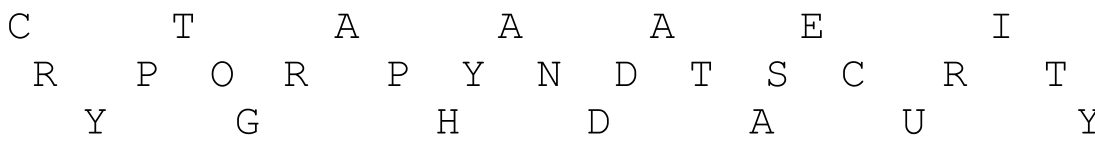
\includegraphics[width=119.70mm,height=41.58mm]{../../images/llm/page_039_img_01.png}%
\end{textblock*}

\end{document}
